%! Author = joaopintosp
%! Date = 8/24/24

% Preamble
\documentclass[11pt, a4paper]{article}
\usepackage[portuguese]{babel}
\usepackage{authblk}

% Packages
\usepackage{amsmath}
\usepackage{siunitx}
\sisetup{locale = DE, per-mode = symbol, range-phrase=--, range-units=single, product-units=single}
\usepackage{graphicx, subcaption}
\usepackage[margin=1in]{geometry}
\usepackage{indentfirst}
\usepackage{setspace}
\usepackage{emptypage}
\onehalfspacing
\setlength{\parindent}{1.25cm}
\setlength{\parskip}{6pt}
\usepackage{booktabs}
\usepackage{lipsum}
\usepackage{wrapfig2}
\usepackage{amssymb}
\usepackage[hidelinks]{hyperref}

\usepackage[capitalise, noabbrev, nameinlink]{cleveref}
\Crefname{figure}{Figura}{Figuras}
\Crefname{equation}{Equação}{Equações}
\Crefname{table}{Tabela}{Tabelas}
\Crefname{section}{Secção}{Secções}

\usepackage[printonlyused]{acronym}
\usepackage[style=apa]{biblatex}
\addbibresource{main.bib}

\author[1]{João Sá Pereira}
\author[2]{Vasco Reis}
\affil[1]{FEUP}
\affil[2]{IST}
\title{Pycharm e \LaTeX}
\date{\today}


% Document
\begin{document}

    \maketitle
    \tableofcontents
%    \listoffigures
%    \listoftables
    \section*{Nomenclature}
%    \renewcommand{\baselinestretch}{0.75}\normalsize
        \begin{acronym}[longest]
        \acro{HTML}{Hypertext Markup Language}
        \acro{t}[$t_{db}$]{dry-bulb temperature \acroextra{[°C]}}
        \end{acronym}
%    \renewcommand{\baselinestretch}{1}\normalsize

    %! Author = joaopintosp
%! Date = 8/25/24
\section{Introdução}\label{sec:introducao}

    The \ac{t} was measured using a thermometer.
    Also, it was verified that the \ac{t} was extremely hot.


    \lipsum[1]

    \subsection{Motivo}\label{subsec:motivo}

    Isto é apenas uma introdução para ver se gosto ou não de utilizar o Pycharm com \LaTeX.
    Pode ser que se torne a minha nova ferramenta de trabalho, sendo que em 2025 começarei a minha dissertação de mestrado.
    \lipsum[1]

    \subsection{Ortografia}\label{subsec:ortografia}

    Será que o Pycharm corrige a ortografia?
    Pelos vistos, sim!
    O Pycharm corrige a ortografia.
    \lipsum[2]

    \paragraph{Parágrafo da Introdução} \lipsum[3]

    \subsection{Figuras e Tabelas}\label{subsec:figuras-e-tabelas}

    Aqui está uma tabela:

    \begin{table}[htb!]
        \centering
        \begin{tabular}{lrr}
\toprule
name & age & height \\
\midrule
FREDERICO & 24 & 170.8 \\
DONATELLO & 45 & 177.7 \\
\bottomrule
\end{tabular}

        \caption{Uma tabela.}\label{tab:tabela}
    \end{table}

    Write some text.
    Como mostrado na Tabela~\ref{tab:tabela}. \lipsum[5]

    Aqui está uma figura.
    Esta é a Figura~\ref{fig:figure}:
    \begin{figure}[htb!]
        \centering
        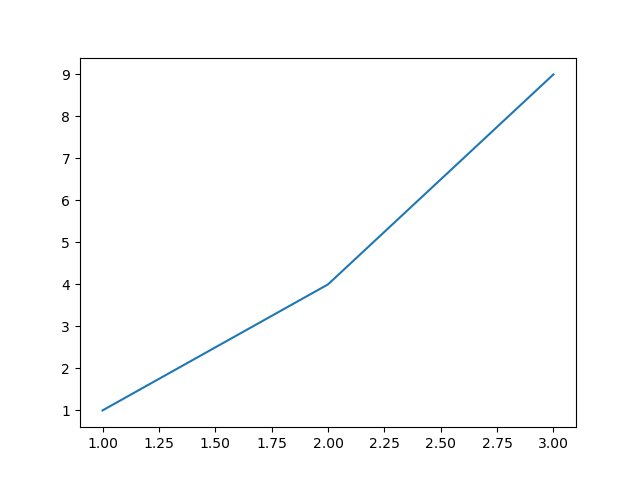
\includegraphics[width=0.5\textwidth]{figures/figure}
        \caption{Isto é um plot.}\label{fig:figure}
    \end{figure}

    \newpage

    Aqui está uma subfigura:

    \begin{figure}[htb!]
        \centering
        \begin{subfigure}[b]{0.45\textwidth}
             \centering
             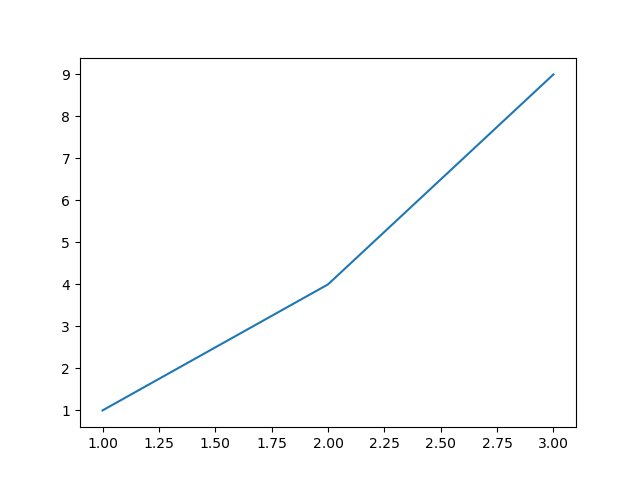
\includegraphics[width=\textwidth]{figures/figure}
             \caption{$y=3\sin x$}
             \label{fig:three sin x}
         \end{subfigure}
         \hfill
         \begin{subfigure}[b]{0.45\textwidth}
             \centering
             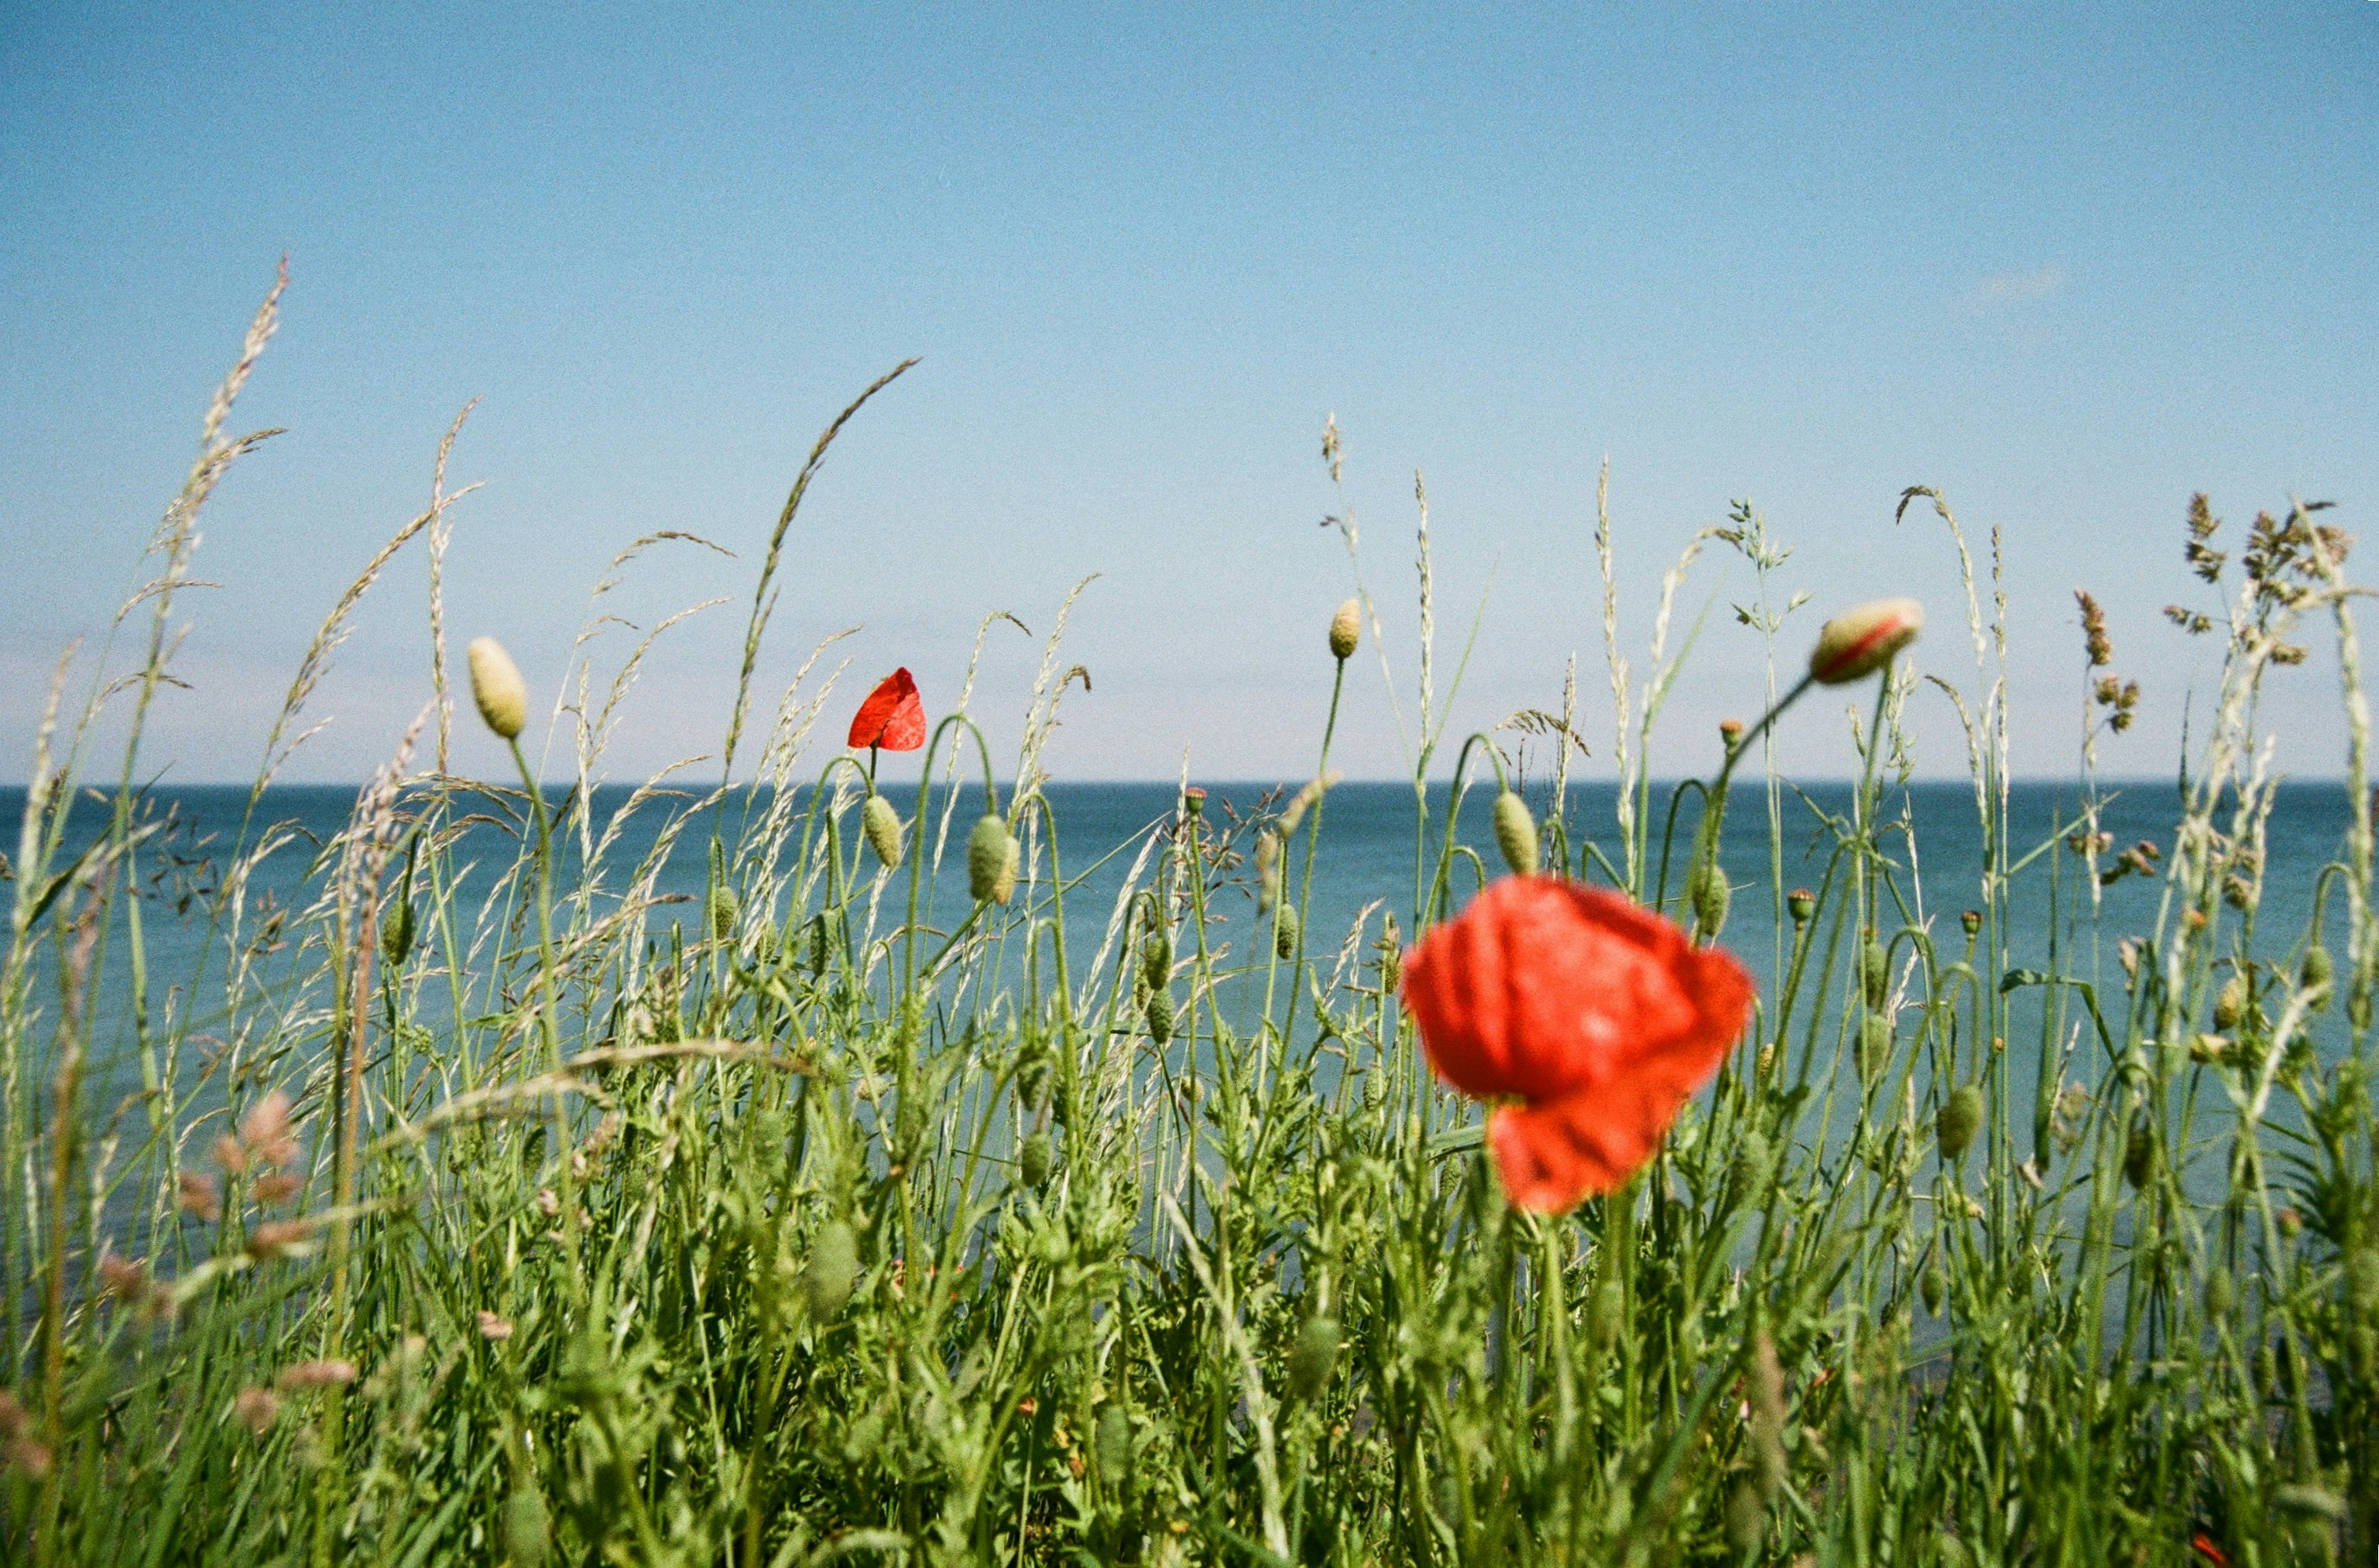
\includegraphics[width=\textwidth]{figures/flores}
             \caption{$y=5/x$}
             \label{fig:five over x}
         \end{subfigure}
            \caption{Duas simples figuras.}
            \label{fig:twographs}
    \end{figure}

    A Figura~\ref{fig:twographs} é composta por duas subfiguras, a Figura~\ref{fig:three sin x} e a Figura~\ref{fig:five over x}.
    %! Author = joaopintosp
%! Date = 8/25/24
\section{Métodos}\label{sec:metodos}

    \lipsum[6-7]

    \subsection{Git e GitHub}\label{subsec:outrometodo}

    Isto é um novo parágrafo, aqui iremos ver como controlar as versões dos documentos utilizando Git e iremos sincronizar este controlo de versões com o github.

    \subsubsection*{Github}

    Aqui submetemos tudo para o Github.

    \subsection{Equações}\label{subsec:equacoes}

    Com o \LaTeX é muito fácil escrever equações, numerá-las e referênciá-las com uma facilidade enorme.
    Aqui está um exemplo de uma equação não numerada:
    \[
        \phi(1) * \phi(2) = \Phi(f) = \int_{-\infty}^{+\infty}  \phi(t) + \phi(t+\tau) \cdot d\tau
    \]

    Aqui está o exemplo de uma equação numerada:
    \begin{equation}\label{eq:classe-c}
        \phi(t) \in C \, \text{ se } \,
        \begin{cases}
            \exists \phi^{(n)} (t) & \forall t,n \\
            \lim_{t \rightarrow +\infty} \left[t^n \cdot \phi(t)\right] = 0
        \end{cases}
    \end{equation}

    \subsection*{Unidades}

    \unit{\m\candela} \par
    \unit{kg.m.s^{-1}} \par
    \unit{\kilogram\metre\per\second} \par
    \unit{\kg\m\per\s} \par
    \unit[per-mode = symbol]{\kilogram\metre\per\ampere\per\second}\par
    \unit{\kilo\gram\metre\per\square\second} \par
    \unit[per-mode = symbol]{\gram\per\cubic\milli\metre} \par
    \unit{\square\volt\cubic\lumen\per\farad} \par
    \unit{\metre\squared\per\cubic\lux} \par
    \unit{\henry\second}

    \subsection*{Números com Unidades}

    \qty{10}{\celsius} \par
    \qty{10}{\degreeCelsius} \par
    \qty{1.23}{J.mol^{-1}.K^{-1}} \par
    \qty{.23e7}{\candela} \par
    \qty[per-mode = symbol]{1.99}{\per\kilogram} \par
    \qty[per-mode = fraction]{1,345}{\coulomb\per\mole}

    \pagebreak

    \subsubsection*{Additional macros for numbers with units}

    \qtylist{0.13;0.67;0.80;1}{\milli\metre}\par
    \numproduct{1.654 x 2.34 x 3.430} \par
    \qtyproduct{10 x 30 x 45}{\metre} \par
    \numrange{10}{20} \par
    \numrange[range-phrase=--]{10}{20} \par
    \qtyrange{0.13}{0.67}{\milli\metre}

    \subsection{Referir as legendas anteriores}\label{subsec:reference}

    Por exemplo, se eu quiser referir a Figura~\ref{fig:twographs}, posso fazê-lo de forma a criar um link que redireciona à coisa referida.

    No entanto, posso também utilizar o pacote \emph{cleveref} que facilita bastante o processo.
    Por exemplo, a \cref{fig:figure}.
    A \cref{eq:classe-c} e \cref{subsec:figuras-e-tabelas}.

\paragraph{Citações} Podemos citar o \textcite{einstein}, da seguinte forma.

Penso que só seja necessário compilar a biblatex caso apareça uma nova citação.
Afinal não, compila tudo
    %%! Author = joaopintosp
%! Date = 8/25/24

\section{Resultados}\label{sec:resultados}

\subsection{Discussão de Resultados}\label{subsec:discussao}

Ou seja, quando for possível acabar com isto.
Espero que seja possível alterar isto de forma a que isto seja viável.
Com o Vim seria capaz de aumentar o meu ritmo de escrita considerávelmente.
Nesta secção iremos apresentar os resultados da nossa pesquisa e analisar os dados obtidos.
Normalmente, num trabalho de investigação, isto tem de ser feito de forma a corroborar as conclusões que irão ser tomadas nas secções finais do presente documento.

Nesse sentido, apresenta-se os seguintes resultados:

\begin{table}[htb!]
    \centering
    \caption{Resultados obtidos.}
    \label{tab:tabela1}
    \begin{tabular}{|c|c|c|}
        \hline
        1 & 2 & 6 \\ \hline
        3 & 4 & 7 \\ \hline
    \end{tabular}
\end{table}

\subsection{Cálculos efetuados}\label{subsec:calculos}

Nesta secção iremos falar sobre os resultados obtidos e apresentados na secção anterior e iremos apresentar os cálculos que nos permitiram chegar a tais resultados.

Começa-se por uma descrição dos trabalhos realizados:
\begin{enumerate}
    \item Perceber o teatro;
    \item Tentar resolver o teatro;
    \item Aperceber-se que não se sabe resolver o teatro;
    \item Desistir de resolver o teatro;
    \item Perguntar ao ChatGPT a resposta;
    \item Discutir os resultados como se fosse eu que os tivesse feito.
\end{enumerate}

\paragraph{Um Diagrama:} Vamos agora observar um diagrama que representa o problema:

\begin{figure}[htb!]
    \centering
    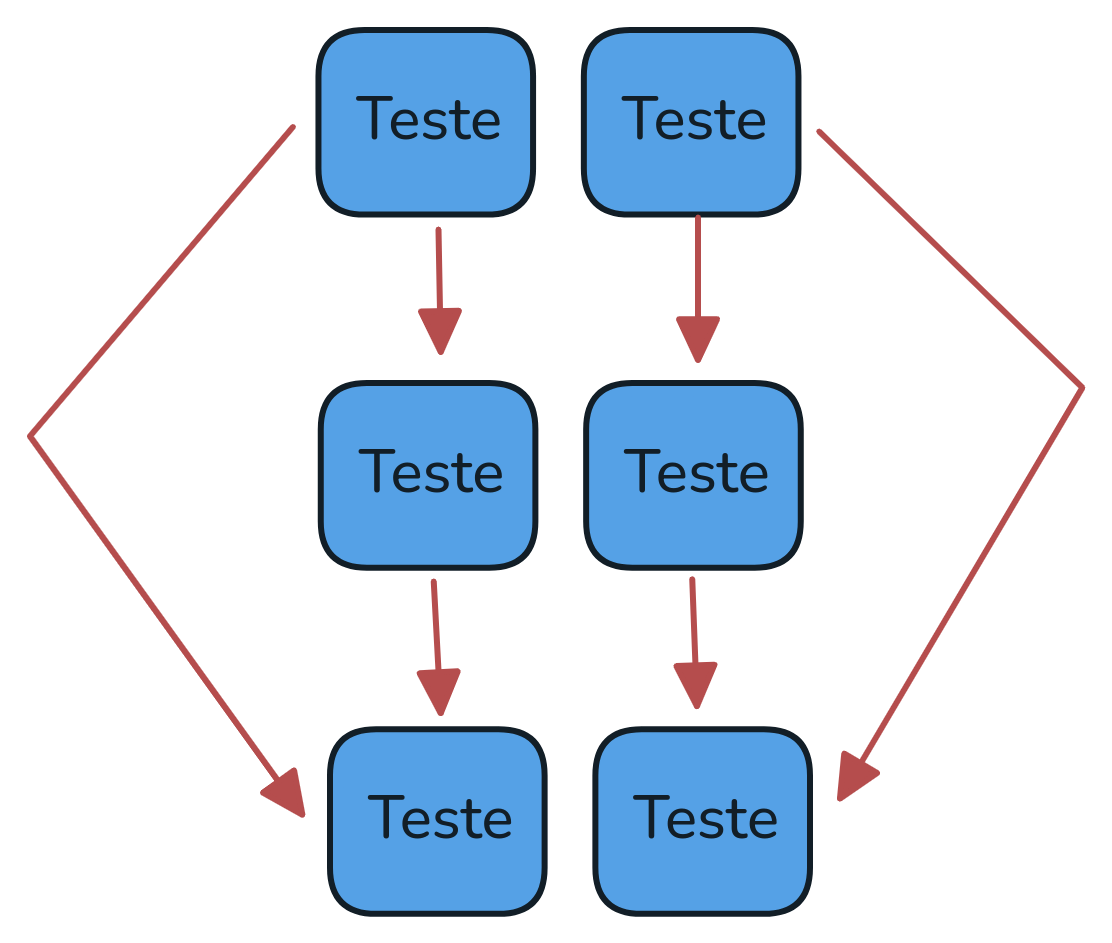
\includegraphics[width=0.5\textwidth]{figures/teste}
    \caption{Isto é apenas um teste.}
    \label{fig:teste}
\end{figure}

\begin{figure}[htb!]
    \centering
    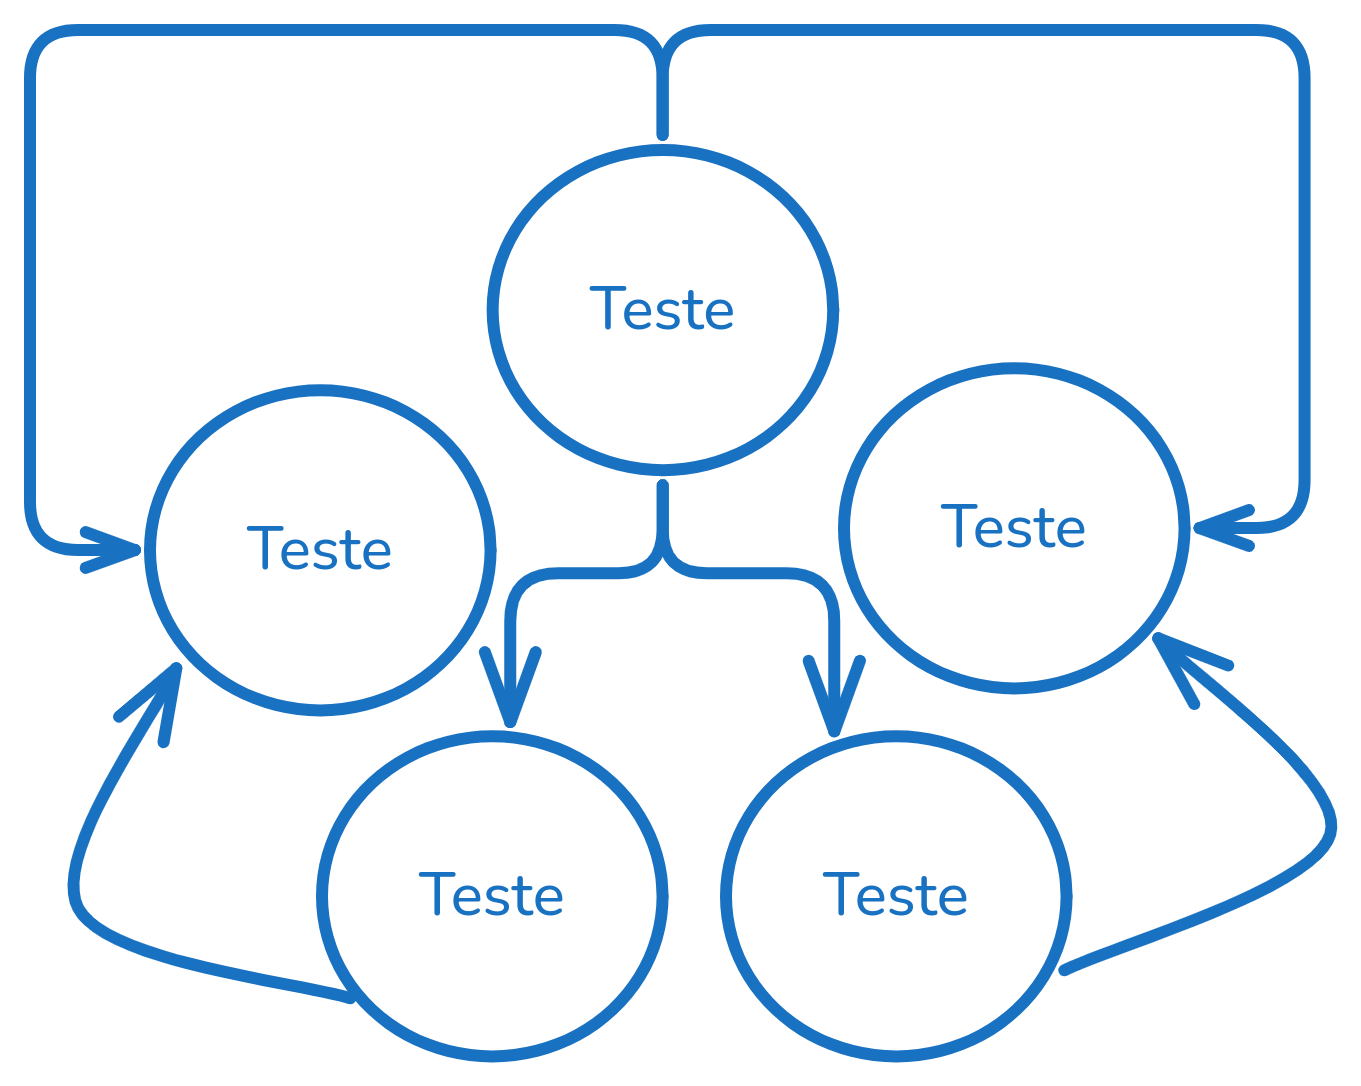
\includegraphics[width=0.5\textwidth]{figures/diagrama}
    \caption{Isto é apenas um teste.}
    \label{fig:diagrama}
\end{figure}

Como podemos ver pelas figuras anteriormente apresentadas, a Figura~\ref{fig:teste} é azul e a Figura~\ref{fig:diagrama} é azul com obrigado.

    
    \nocite{*}
    \printbibliography


\end{document}
